\documentclass[]{final_report}
\usepackage{graphicx}
\usepackage{hyperref}


%%%%%%%%%%%%%%%%%%%%%%
%%% Input project details
\def\studentname{Oraz Ospanov, Asset Malik, Andrey Yershov}
\def\projecttitle{Data-Driven Control for DC Motors}
\def\supervisorname{Do Duc Ton}

\begin{document}

\maketitle

\pdfbookmark[0]{Table of Contents}{toc}
\tableofcontents
\newpage

%%%%%%%%%%%%%%%%%%%%%%
%%% Your Abstract here

\begin{abstract}

\textbf{\textsl{Insert abstract here (see details later in these guidelines).}}

\end{abstract}
\newpage

%%%%%%%%%%%%%%%%%%%%%%
%%% Acknowledgments

\chapter*{Acknowledgments}

In your Acknowledgments section, give credit to all the people who helped you in your project.

%%%%%%%%%%%%%%%%%%%%%%
%%% Introduction

\chapter{Introduction}
The modern control theory, also known as Model Based Control has been used both for linear and non-linear systems extensively since 1960. The Model Based Control is, as could be guessed from it's name, relies solely on the model of the plant for further controller design. However, there is usually no chance of creating an exact plant model for the system, as well as no efficient way of creation high accuracy plant model using the classical model based control \cite{hou2013model}. Moreover, the possible plant model errors have to be considered when designing the controller from the plant model, what requires additional resources and time to provide robustness of the controller. All of the used control design methods heavily rely on the assumptions of an accurate plant model design. This means that in case if unmodeled dynamics occurs, the controller is believed to be unable to provide further handling of the dynamics. As could be seen in Fig. \ref{fig:mbcsctruct}, the Model Based Controller design starts from the assumptions about the model plant and is directed at regulation of the plant \cite{hou2013model}.

\begin{figure} [h!]
\centerline{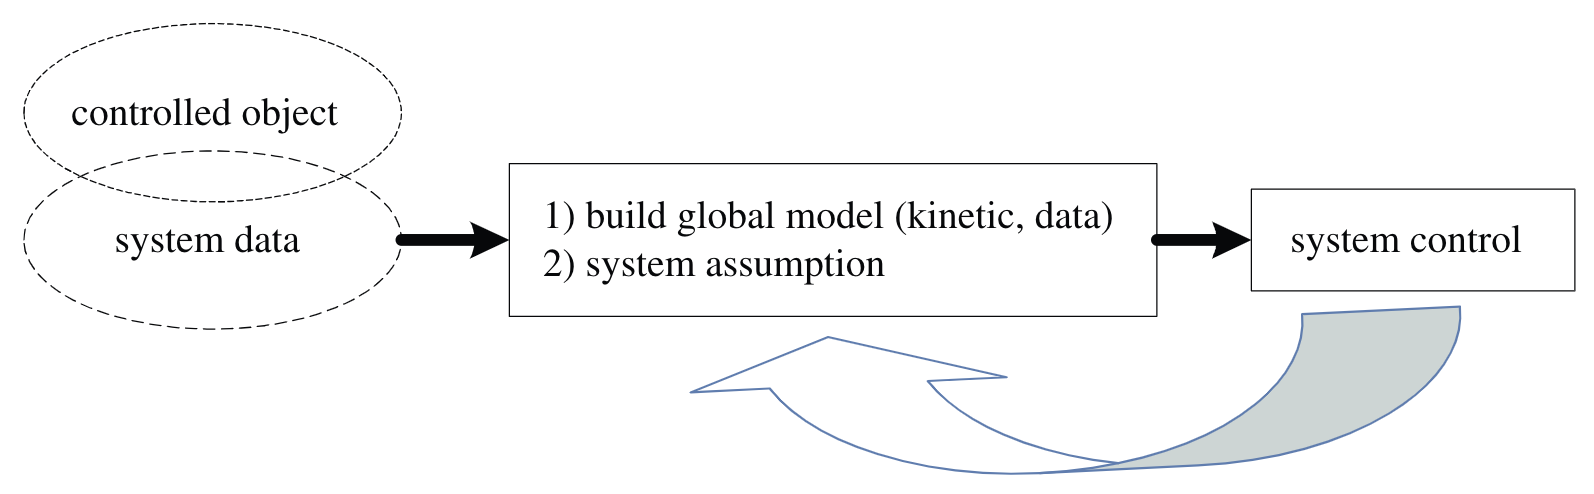
\includegraphics[width=.75\textwidth]{Screenshots for paper/1.png}}
\caption{Common structure of the Model Based Control \cite{hou2013model}}
\label{fig:mbcsctruct}
\end{figure}

The recent development of highly capable machine learning techniques and frameworks.

Data-Driven control for various purposes is becoming the superior method in systems where the model is not available or is changing over the course of life cycle, i.e. adaptability is necessary. Data-Driven controller design method allows to bypass the tedious system identification step. However, as every machine learning problem, it requires big amounts of data. The data gathered from the system behaviour is used to identify the controller. In this paper, we investigate the application of data-driven control to the control of DC motor drives and experiment with data-driven controller estimation using reinforcement learning.

\chapter{\label{chapter2} Related Work}


The article written by Naung et al. \cite{naung2018a} is closely related to our work by the research aims and methods. Authors present Data-Driven Control used for system parameters identification, an approach that we are planning to use. The main goal of the paper is to perform system identification utilizing the data driven system control of the DC motor, with ultimate generation of the transfer function suitable for robust control of the plant. For this purpose, authors use MATLAB to create the Simulink model of the DC motor (Figure \ref{fig:dcsimulink}) and calculate the proportional-integral-differential (PID) controller according to the obtained models.

\begin{figure} [h!]
\centerline{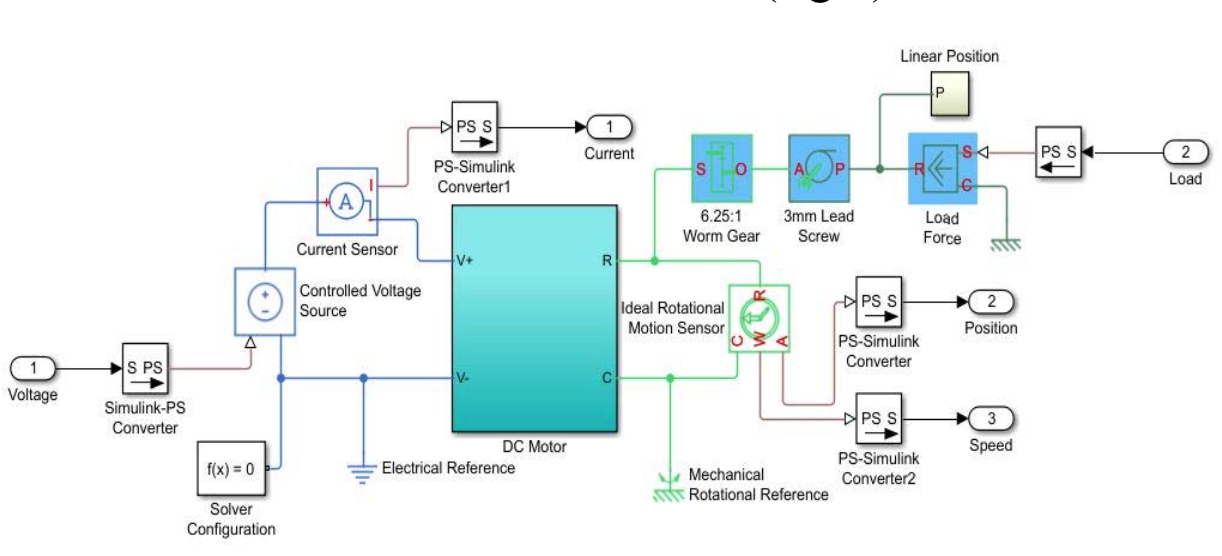
\includegraphics[width=.75\textwidth]{Screenshots for related work/1.png}}
\caption{Simulink diagram of simscape physical plant DC motor \cite{naung2018a}.}
\label{fig:dcsimulink}
\end{figure}

Authors compare the performance of the nonlinear autoregressive exogenous inputs (NARX) artificial neural network and nonlinear black-box model structures, summarized in Figure \ref{fig:pidcomparison}. They conclude that the proposed control method performs with acceptable accuracy and is utilizable with more complex dynamic systems. 

\begin{figure}
\centerline{
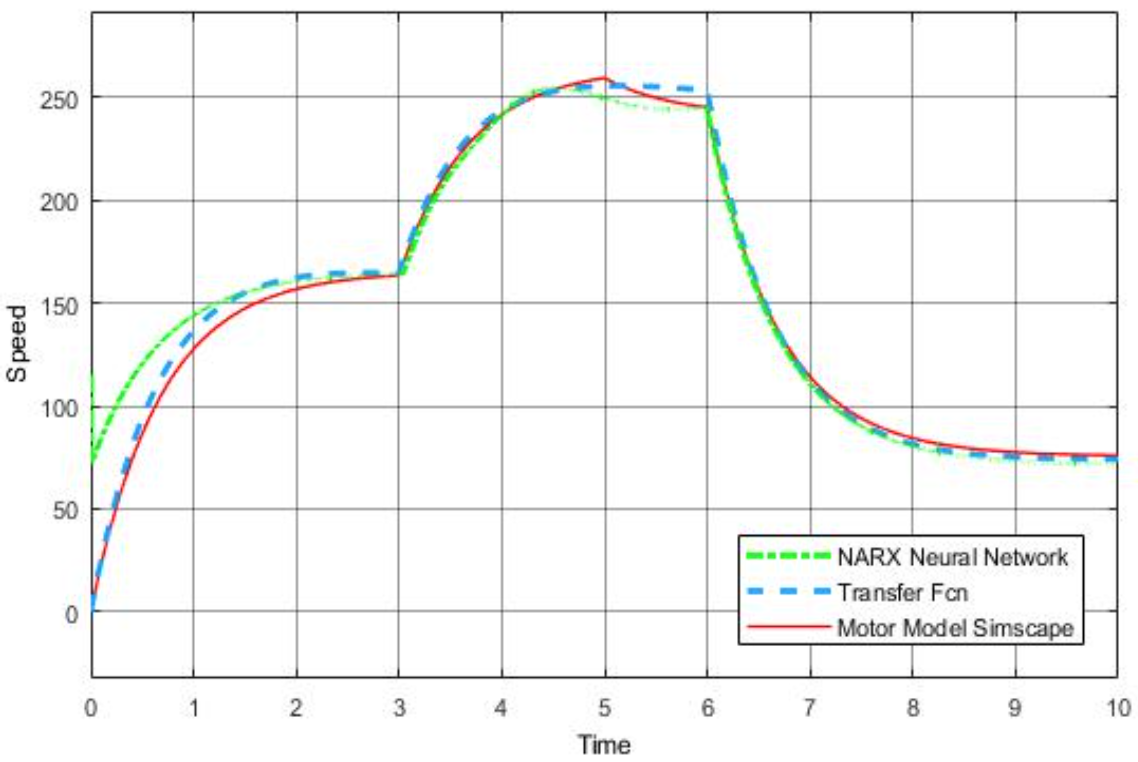
\includegraphics[width=.47\textwidth]{Screenshots for related work/2.png}\hfill
\label{NARX ANN}
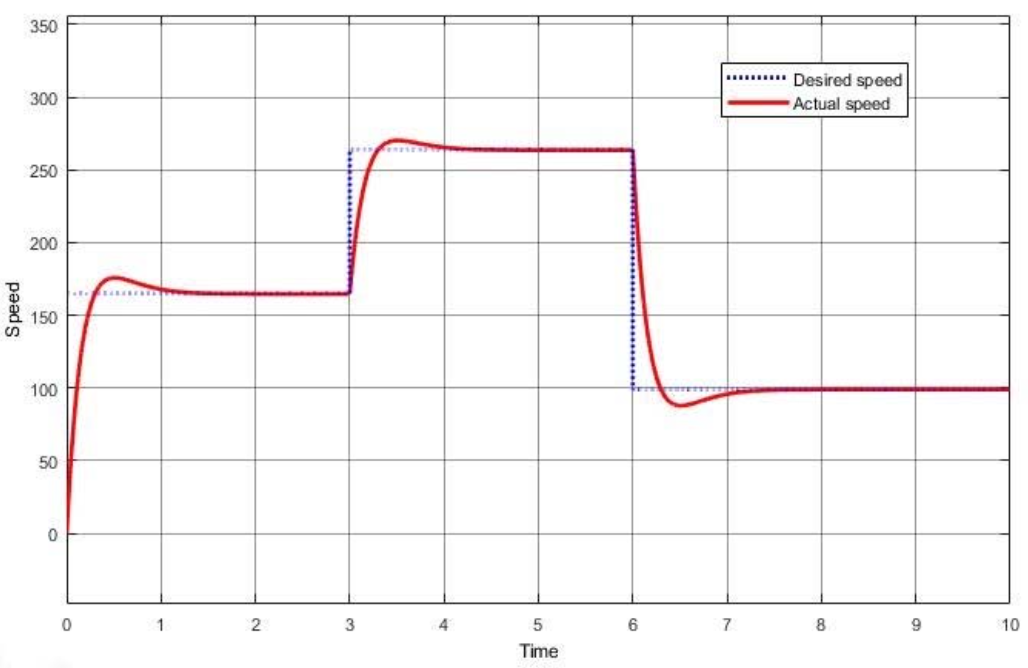
\includegraphics[width=.49\textwidth]{Screenshots for related work/3.png}
\label{PID controller}
}
\caption{Results of the speed response of the DC motor using NARX Neural Network and PID controller \cite{naung2018a}.}
\label{fig:pidcomparison}
\end{figure}

Coulson, Lygeros, and Dorfler introduce novel data-enabled predictive
control (DeePC) algorithm \cite{coulson2019data}, that utilizes real-time feedback of the system, and is able to drive the system along a desired trajectory with given system constraints. The DeePC  algorithm  was  applied  to unknown linear time-invariant (LTI)  system  and was compared to classical Model  Predictive  Control (MPC) algorithm. Authors state that the DeePC was created with thinking from a behavioural systems theory perspective. The algorithm description is provided in both mathematical proof form and a pseudo-code description of the algorithm steps. As an example of sophisticated nonlinear application of the DeePC, a case, a regularized version of the algorithm was simulated on  stochastic nonlinear quadcopter dynamics, illustrating its capabilities beyond deterministic LTI systems - figure \ref{fig:quadsim}.

\begin{figure} [h!]
\centerline{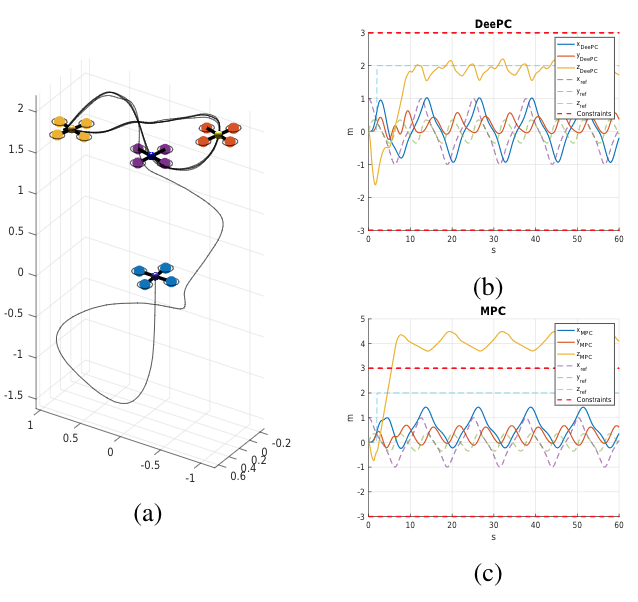
\includegraphics[width=.75\textwidth]{Screenshots for related work/5.png}}
\caption{Figure (a): three dimensional plot of the trajectory of the quadcopter at different instances of time controlled with DeePC.  Figure  (b)  and  (c):  trajectories  of  the  spatial  coordinates  when  controlled  by  DeePC  and  MPC,  respectively. The horizontal red dashed lines represent constraints.
\cite{coulson2019data}}
\label{fig:quadsim}
\end{figure}

A recent work by Carlet et al. \cite{carlet2020data} utilizes the aforementioned DeePC algorithm in a setup with motors. This is an important article for our project, as it explores predictive current control for permanent  magnet synchronous motor drives - a topic closely related to ours. Authors utilize two  of  the  most  popular data-driven   algorithms - the   Subspace Predictive  Control  algorithm  and  the  Data-Enabled  Predictive Control  algorithm. Current  controller  design  procedure for both methods is discussed and presented in detail. Simulation results are reported to be comparably robust and with strong correlation for both of the unconstrained  and  constrained  versions  of  the  data  driven  methods, as it could be seen in figure \ref{fig:controllercomp}.

\begin{figure} [h!]
\centerline{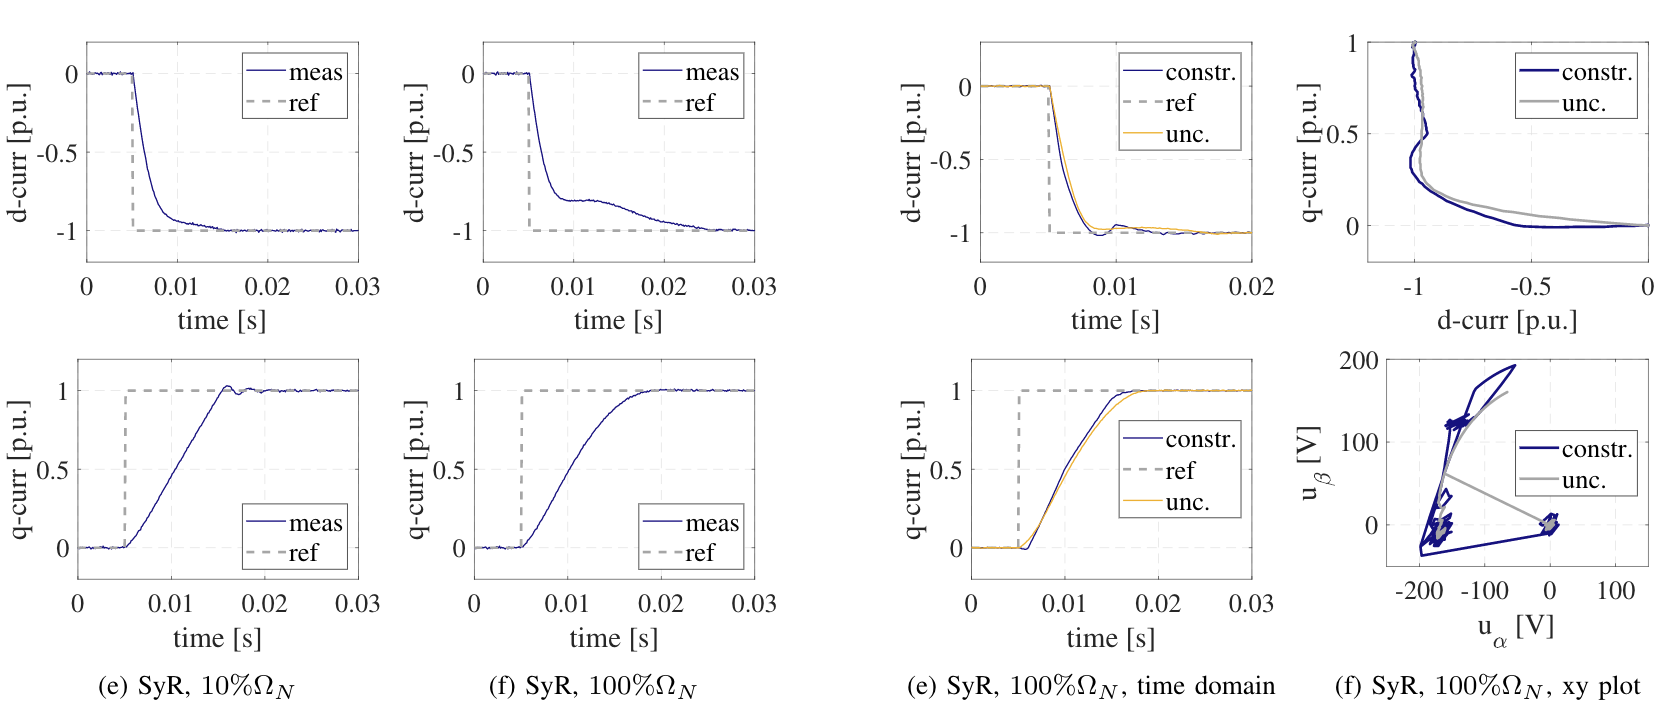
\includegraphics[width=.95\textwidth]{Screenshots for related work/4.png}}
\caption{Step response of SPC data-driven current controllers
\cite{carlet2020data}}
\label{fig:controllercomp}
\end{figure}

Hou and Wang created a canonical survey paper in the field in 2013 \cite{hou2013model}. Almost every other related work cites this paper, as it contains fundamental definitions for the Data driven control and its applications. The paper begins with a brief description and comparison of Model based control theory and Data driven control theory. Motivation for the data based control is stated as well. Further, they state the focus of data-driven control theory in terms of objects that could be controlled with the use of it. For the rest of the survey paper authors explore the recent advances in DDC and discuss the perspectives of future related work. They conclude with categorization of different available Data-driven techniques according to required usage. However, the survey's drawback is that most of the methods are currently outdated, as this is a fast evolving field. The general introductory information provided by the authors is nevertheless valuable.



Next article by Hanke, Wallscheid and Bocker \cite{hanke2019continuous}  introduces Permanent Magnet Synchronous Motor ripple avoidance using DDC. It also compares three types of linear controllers and the input/output data.

\begin{figure} [h!]
\centerline{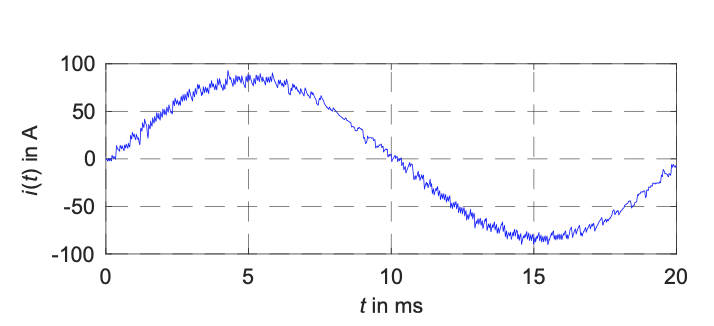
\includegraphics[width=.75\textwidth]{Screenshots for related work/Asset p1/Asset p1p1.png}}
\caption{CCS-MPC at 60A
\cite{hanke2019continuous}}
\label{fig:p1p1}
\end{figure}

\begin{figure} [h!]
\centerline{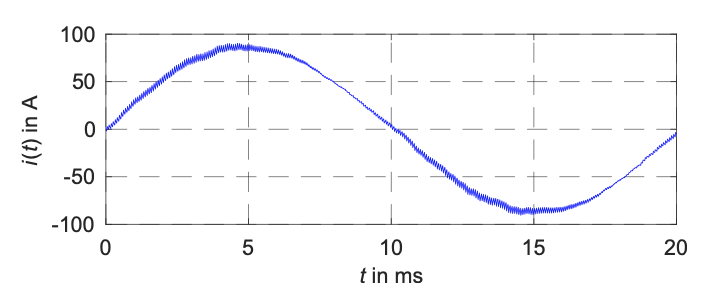
\includegraphics[width=.75\textwidth]{Screenshots for related work/Asset p1/Asset p1p2.png}}
\caption{FOC at 60A
\cite{hanke2019continuous}}
\label{fig:p1p2}
\end{figure}

\begin{figure} [h!]
\centerline{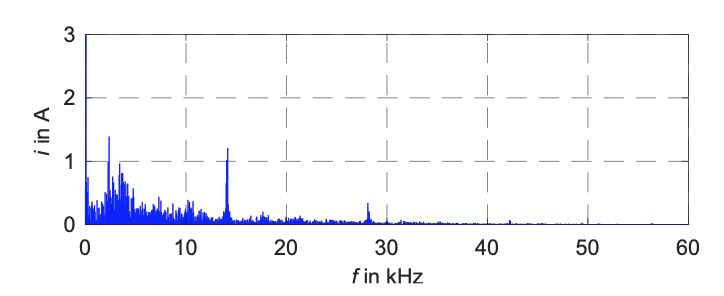
\includegraphics[width=.75\textwidth]{Screenshots for related work/Asset p1/Asset p1p3.png}}
\caption{CCS-MPC at 60A
\cite{hanke2019continuous}}
\label{fig:p1p3}
\end{figure}

\begin{figure} [h!]
\centerline{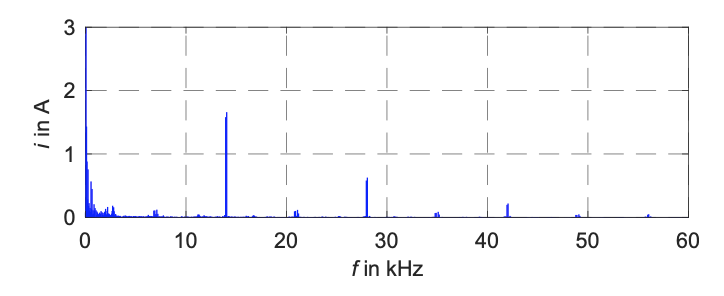
\includegraphics[width=.75\textwidth]{Screenshots for related work/Asset p1/Asset p1p4.png}}
\caption{FOC at 60A
\cite{hanke2019continuous}}
\label{fig:p1p4}
\end{figure}

We can clearly see that total harmonic distortion of the FOC system is smaller and that CCS-MPC only better at those special harmonics of the three phase system. 

Article \cite{de2019a} discusses the important attributes for systems with data-driven control: Stabilization, Optimality, and Robustness. Authors argue that it is possible to create a linear approximation of a non linear closed loop system using only data-dependant linear matrix equations. 

Article \cite{rosolia2018a} explores the ability of the data-driven system to adapt and thus improve its performance in case of changes of parameters. The author argues that it is possible to have a learning model that could be started without correct initial state and even learn from data without diverging back from better state, which is backed by simulation. Each discreet step of the controller is used as an iteration for the learning algorithm. Model Predictive Control (MPC) was chosen as a back-bone for the closed loop control and re-applied as MPC for Batch processes (iterations) and then replaced by LQR as LMCPC. 

\begin{figure} [h!]
\centerline{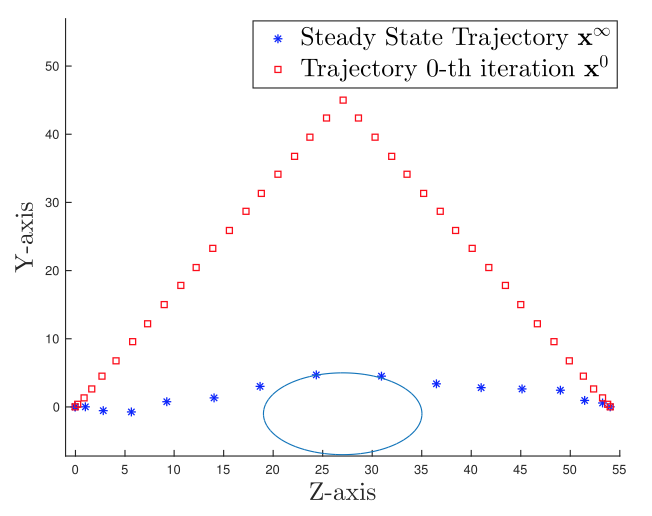
\includegraphics[width=.75\textwidth]{Screenshots for related work/Asset p1/Asset p2p1.png}}
\caption{SS positions over ZY plane
\cite{rosolia2018a}}
\label{fig:p2p1}
\end{figure}


Article \cite{bu2018a} analyzes the behavior of data-driven control in the extreme case of output saturation. This paper also uses a linear system approximation approach with dynamic linearization, but also applies assumption that the system has an output saturation. This does increase the tracking performance but decreases the resting time of the closed loop system. 

Article \cite{pravallika2021a} is an official MATLAB tutorial to DDC, which we follow with our designed controller simulation in the beginning of our project.

A recent article \cite{Berberich_2020} overviews a problem of state-feedback controllers for discrete-time linear time-invariant systems, based directly on measured data. This paper presents the robust methods for data-driven control in which the stable closed-loop performance is guaranteed even in presence of noise in data. The design of state-feedback controllers is based on the parametrization technique analyzed in \cite{de2019a}, particularly the application of robust control techniques to the parametrization, which results in stable performance of the closed loop control with noisy inputs.

In the paper \cite{piga2017direct} a data-driven approach is used to design a hierarchical controller which includes the inner and outer controllers to enhance the overall performance of the inner controller. The evaluation of the effectiveness of this type of method is done by means of simulation and practical experiments. Basically this paper proposes the implementation of the outer Model Predictive controller used for improving the performance of an inner closed loop controller. In such a way it is not only improves the overall performance of the system, but also takes care of constraints imposed on inputs and outputs. Figure \ref{fig:hierarchicalcontroller} shows the resultant hierarchical controller, in which it can be seen that the outer Model Predictive controller tracks the input and output variables and operates on the reference signal applied to the inner loop in order to satisfy the constraints imposed on inputs and outputs of an overall system as well as improve on the system performance. To test the results the simulation of a servo positioning system in dc motor was used. The inner loop controller design resulted in the following performance shown in figure \ref{fig:innerloopcontroller}. However because of the lower degrees of freedom of the controller the controller could not obtain the faster dynamics and thus resulted in slow dynamics with the rise time of about 4 s. Adding the model predictive controller resulted in much better performance as shown in figure \ref{fig:controllerwithMPC} below. The rise time resulted in 1.3 s, which is about 3 times as much faster as the previous result. 

\begin{figure} [h!]
\centerline{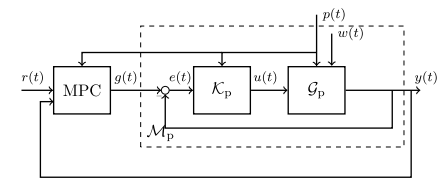
\includegraphics[width=.75\textwidth]{Screenshots for related work/constraint_data_driven_control_screenshot1.png}}
\caption{Proposed hierarchical control architecture
\cite{piga2017direct}}
\label{fig:hierarchicalcontroller}
\end{figure}

\begin{figure} [h!]
\centerline{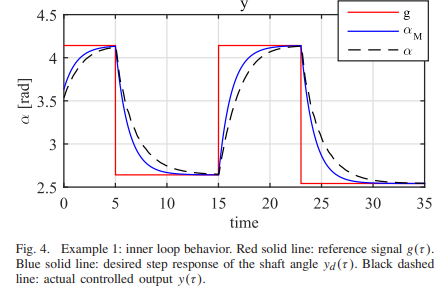
\includegraphics[width=.75\textwidth]{Screenshots for related work/constraint_data_driven_control_screenshot2_innerloop.png}}
\caption{Inner loop behaviour
\cite{piga2017direct}}
\label{fig:innerloopcontroller}
\end{figure}

\begin{figure} [h!]
\centerline{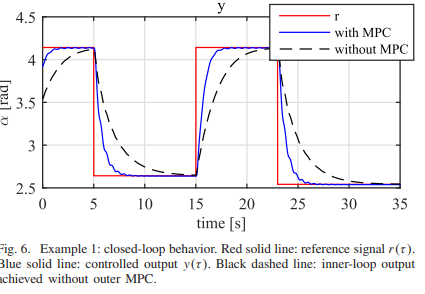
\includegraphics[width=.75\textwidth]{Screenshots for related work/constraint_data_driven_control_screenshot2_usingMPC.png}}
\caption{Closed loop behaviour with added MPC
\cite{piga2017direct}}
\label{fig:controllerwithMPC}
\end{figure}

A PhD thesis \cite{kergus} explores a Data-driven model reference control in the frequency-domain. 

An article \cite{CAMPESTRINI20172628} deals with Data-Driven (DD) control design in a Model Reference (MR) framework. 

Article \cite{vuillemin2019hybrid} shows a discrete-time control-law from frequency-data of a continuous-time plant so that their hybrid interconnection matches a given continuous-time reference model up to the Nyquist
frequency. 

Article \cite{Waarde2020} Data Informativity: A New Perspective on Data-Driven Analysis and Control

\chapter{Preparing your Project Report}

Report writing is an important skill. No matter what field you are engaged in, you will almost certainly find it necessary to be able to write a clear report on your work. If you have a talent for technical writing, you will no doubt find it an easier task. However, it is a skill that can be acquired with practice and it is an essential part of your project work. Be sure to allow yourself enough time to write the report; the process generally takes {\bf at least} two weeks. 

The following sections suggest how to approach the structuring and writing of your report. It is not carved in stone; feel free to adjust this to suit your own particular project/style, but make sure your report is well written.

\section{Create a Report Structure}

The first step is to produce a draft table of contents, showing how the entire report is to be structured into chapters, sections, and even subsections. Annotate each item with the purpose it is to serve in the overall report, and its anticipated length in pages. When you have done this ask yourself the following questions:

\begin{itemize}
\item Is there a logical flow through my report? If it does not flow logically at this high-level stage, it certainly will not flow well in the end either. Move sections around until you feel there is a logical thread running through the document.
\item Have I written about all the important issues? Pull yourself back from the report and think about the project in general. You should not write about {\sl everything} you did (this is a report, not a diary) but do not omit any vital sections either.
\item Are the issues that I have written about important? You have probably written sections that should really be omitted. It is tough to cut out a section that you have laboured over, but dross in a report has a very negative effect on overall quality.
\end{itemize}

Once you have a sound overall structure, you can start writing sections knowing that they fit in to an overall plan. You will know how much preparatory material will have preceded each section, and you will know to what extent it is expected to lay the groundwork for later sections. You may find that you have to change the structure later in the writing of the report. As with software, the later you change the design, the more work it entails.


\section{Typical Structure of your Report}

The details of the structure of your report will of course depend on the content and nature of the particular project you are working on. Generally you should break down the report into approximately six chapters. One possible template you could use is detailed below, but remember that this template is only for guidance. You may decide to merge some chapters, or have an extra core chapter. It all depends on your project and how you wish to present it.

\subsection{Title page, Table of Contents, and Acknowledgements}

The title page should state at least the project title, the name of your supervisors, and all names of the students. A Table of Contents is essential, but should be produced by the word processing package you are using. In your Acknowledgments section, give credit to all the people who helped you in your project.


The Introduction chapter introduces the project and describes the general subject area of the project. Topics it may contain include:

\begin{itemize}
\item A discussion of the original aims of the project, and the modified aims if appropriate;
\item The scope of the project and a general justification for the work undertaken, perhaps providing a brief background description;
\item A description of the structure of the report, i.e., a road map for the reader.
\end{itemize}


\subsection{The Abstract}

What is an abstract? The abstract should provide a short overview of your project that enables a reader to decide if your report is of interest to them or not. It should be concise, to-the-point and interesting. Avoid making it read like a verbose table of contents! Avoid references, jargon or acronyms, as the reader may not be familiar with them. An abstract usually contains a brief description of:

\begin{itemize}
\item The project and its context;
\item How the project work was carried out;
\item The major findings or results.
\end{itemize}

The main thing to remember is the principle that the abstract must be short, and a person reading it should be able to determine if they want to read more. Your abstract has to be \textbf{between 150 and 250 words.}


\subsection{Chapter 1: Introduction}

This chapter introduces the project and describes the general subject area of the project. Topics it may contain include:

\begin{itemize}
\item A discussion of the original aims of the project, and the modified aims if appropriate;
\item The scope of the project and a general justification for the work undertaken, perhaps providing a brief background description;
\item A description of the structure of the report, i.e., a road map for the reader.
\end{itemize}

\subsection{Chapter 2: Background Research}

The contents of this chapter depend on the nature of your project. If you are working on a research-oriented project, then you will present the research landscape within which your project is being conducted and consider approaches that have been adopted by other researchers. In a development project, you may describe the domain in which you are working and the technologies and programming tools you are using. Tutorial-type descriptions are never appropriate, but if you are using a specialist tool, e.g., a parser generator, it is reasonable to provide a section that describes the tool at a high level.


\subsection{Chapters 3 and 4: The Core Chapters}

These are the principal chapters of your report and their structure will vary from project to project. The aspects of your project that you will describe in these chapters include:

\begin{itemize}
\item A detailed account of how you approached your project, i.e. the strategy you employed. This should be at a high level, separate from design and implementation issues.
\item A discussion of the design aspects of your project. Include here a discussion of interesting problems you encountered and the alternative solutions you considered.
\end{itemize}

Use the appropriate notations and formalism in this chapter! Everything you have studied in your degree is relevant here. If there is a crucial algorithm at the centre of your project and its performance is important, attempt to provide an analysis of its complexity. If you are describing a complicated set of conditions, do not write it in English, use first-order logic. If you have performed an object-oriented design (as most of you will), use a UML Class Diagram to give a high level view of your program. If you are describing how objects interact to perform some task, use a UML Sequence or Interaction diagram. Do not mindlessly produce ``documentation'', but think about what you want to communicate to the reader and don't be afraid to use the most appropriate method of doing so.

\subsection{Chapter 5: Detailed Design and Implementation}

In doing your project work, a lot of time will be spent on detailed design and implementation. The nature of programming is that it is a very time-consuming task, and even for experts a ``silly" run-time error may take days to correct. In spite of this, this chapter should not be the main focus of your report. Make it clear what implementation technology you used and discuss any interesting implementation issues that arose. For example, if you were using a particular data structure that had to be optimized in a certain way to be suitable for your project, describe it in this chapter. On the other hand, if you used an obvious/standard approach, then there is no need to devote much space to it.

\subsection{Chapter 6: Testing/Evaluation}

You may decide to merge this chapter with another, but I have described it as a separate chapter as it is very important in its own right.

If the focus of your project is the development of a piece of software, then you should address the issue of how you demonstrate it to be correct. Formal proof is applicable in a small number of cases, but more commonly rigorous testing is required. You will not have time to really test your software in the way that industrial software is tested. However it is important to show that you have taken a methodological approach to testing and that you have tested your software in such a way that you are justified in having some confidence that it is correct. Any Software Engineering text will provide you with the basics of software testing; contact me if you want some notes on the topic.

Another type of project involves designing a heuristic or approximate solution to a challenging or ill-defined problem, e.g., to develop a junk mail filter or to mine a certain type of data from the web. In this case the precise desired behaviour of the software is hard to specify (what is junk mail anyway?), so it is more appropriate to describe how you evaluated the solution. This will involve running a number of experiments and presenting the results. As with testing, this is a complex area that you should spend some time coming to terms with. Consult~\cite{DAWSON:2000} for some excellent advice on how to present the results of your experiments.


\subsection{Chapter 7: Conclusions and Future Work}

If you are writing this chapter bleary-eyed and caffeined-up on the day of submission, you are not going to do your project justice. This is a vital chapter in the assessment of your work. Academics, in getting the feeling for any type of report, will typically read the introduction and conclusions first. Your conclusions should not read like ``I did all this stuff, it went great, and here's other stuff someone else might do.'' This chapter should cover the following areas:

\begin{itemize}
\item {\sl Conclusions:} In a research-oriented project you will state the overall conclusions you have come to. In a development project there may not be a conclusion as such, so just state what has been achieved. Be very critical in this section. Describe the weaknesses of your approach and avoid making unwarranted conclusions.
\item {\sl Future Work:} Think carefully about how your work might be extended or applied to another domain. There will probably be some obvious extensions. If you are able to propose some interesting ideas that are not immediately apparent, this demonstrates that you have a clear understanding of the field.
\end{itemize}

It is good scientific style to make strong statements. If a certain statement is warranted by the results of your project, don't be afraid to make it. Strange though it may seem, a strong statement that turns out to be wrong is better than one that is vague and wishy-washy. The former can lead to a lively debate where the truth may emerge, but the latter will produce meaningless agreement, because it ultimately says nothing.

\subsection{References}

Use one consistent system for citing works in the body of your report. Several such systems are in common use in textbooks and in conference and journal papers. Ensure that any works you cite are listed in the references section, and vice versa. Word-processing packages will manage the referencing for you, and be sure to make use of this facility. It may take more time in the beginning, but at the end of the write-up it will certainly have saved you a lot of time.

You may instead opt for a bibliography, which is a list of material (books, papers, web resources) that you have read in preparing your project. The bibliography must be annotated, i.e., for each entry you must provide a paragraph summarizing the work and stating why it is relevant to your project.

\subsection{Appendices}

Material that you want to include in your report, but that is not directly relevant to the main thread of your report, can be put in an appendix. Possible examples include program/code listings, detailed test results, user guides etc. In most cases, appendices are not necessary and it is only in an exceptional case that it is useful to provide a code listing.

Remember that material in the appendix counts towards report length, so do not exceed the limits defined earlier.


\section{Order of Writing}

The previous section dealt with one possible logical structure for your report. The order in which your write it all is another issue. There are no fixed rules here. Some people like to write notes throughout the project, so when it comes to writing the final report, they already have a lot of material prepared. This is a very valid idea, but avoid wasting time writing very polished notes during your project work. The notes/sections you write can be quite rough, and only in the final report do you bring them up to full report quality. The reason for this is that you may have to tailor them considerably to fit the context of the report, and this will mean that much of the polishing will have gone to waste.

Assuming you have created a report structure as described earlier, a good way to continue is to write the introduction in draft form. You already have an introduction from the interim report, so you can flesh this out. The reason why you write this in draft form is that you are not yet sure what you are introducing! Only when the later chapters are completed can you return and finish the introduction.

Now the Background chapter of the interim report can be revisited and improved for the final report. Again, you may find that when you write the core chapters later, that some of the background work becomes irrelevant and can be removed. This may seem like wasted effort, but if it results in a tighter Background chapter, do it.

Next are the Core chapters, followed by the design and testing chapters. When these are complete, you are in a position write your Conclusions chapter, and to return to the Introduction and Background chapters and bring them to completion. Finally, write the abstract.

The next step depends on how much time you have left. Ideally you will reach this point where you have a first full draft with at least a week to go. Proofread the report yourself, and pass it on to other people who can help you with the English grammar. Take a rest yourself, so you can return to it in a day or two and re-read the report with a fresh mind.

Note that at this late stage you can only make local improvements to the report. It is too late for major overhauls, so at this point the importance of creating a good overall structure becomes clear. If you have started with a good structure, you can aim to create an excellent finished product. However if your initial structure was awkward, the final report will not read well no matter how you tweak it.

\section{Other Advice}

This section contains a number of guidelines that are worth bearing in mind when writing.


\subsection{Continuity}

You may not realize this, but a good academic paper or report, like any good novel you have read, tells a story. It is valuable to keep this in mind when you are writing your report. There should be a storyline running through your report and you should make it easy for the reader to hang on to this storyline:

\begin{itemize}
\item At the end of the introduction provide a short description of the layout of
the remainder of the report.
\item Start every chapter with a brief recapitulation of the story so far, and an
overview of what the chapter is going to add.
\item Finish every chapter with a summary of the material in that chapter, and
state how it relates to what follows.
\end{itemize}

In the core chapters, you should take care to make absolutely clear the logical connection between the overall project design and the detailed problems you discuss. If the reader is mired in a detailed description of your solution to some intricate problem, they will be encouraged to persevere if you have clearly indicated its place in the overall project.

This continuity material may sound unnecessary and redundant, but it is useful to the reader. It may help for you to imagine that the reader is coming back to your report after a break of a few days: they will be greatly assisted by occasional reminders of what has already been said.

\subsection{Presentation Issues}

Focus on expressing your ideas clearly. Part of your report is of course its physical layout and use of diagrams. Try not to put too much time into this. If you use the provided \LaTeX\ template, it will help you focus on the content as opposed to the form. Simple diagrams are fine, and avoid the use of colour unless it really contributes something in particular. Do not bother with tricks like adjusting spacing or margins or fonts in order to make your report bigger or smaller.

Most final reports will contain a mixture of figures and charts along with the main body of text. The figure caption should appear directly after the figure as seen in Figure~\ref{fig:logo} whereas a table caption will appear directly above the table. Figures, charts and tables should always be centered horizontally. 

\begin{figure}[h]
\centering
\fboxsep 2mm
\framebox{
	
\includegraphics[width=6cm]{logo} 
	
\includegraphics[width=3cm]{logo} 
	
\includegraphics[width=1.5cm]{logo} 
	
\includegraphics[width=0.75cm]{logo} 
	
\includegraphics[width=0.375cm]{logo}
}
\caption{\label{fig:logo} Logo of NU displayed at various size.}
\end{figure} 

If you wish to print a short excerpt of your source code,  ensure that you are using a fixed-width sans-serif font such as the Courier font. Your code will be properly indented and will appear as follows:

\begin{verbatim}
static public void main(String[] args) {
  try  {
    UIManager.setLookAndFeel(UIManager.getSystemLookAndFeelClassName());
  }
  catch(Exception e) {
    e.printStackTrace();
  }
  new WelcomeApp();
} 
\end{verbatim}


%%%% ADD YOUR BIBLIOGRAPHY HERE
\newpage
\bibliographystyle{ieeetr}
\bibliography{bibliography} 

\label{endpage}


\end{document}

\end{article}
